%%=============================================================================
%% Kosten
%%=============================================================================

\chapter{Kosten}
\label{ch:kosten}

De kosten van EventSourcing kunnen opgedeeld worden in 3 grote delen. Het eerste deel gaat over de fysieke infrastructuur kosten die EventSourcing met zich meebrengt. Het opslagen van alle belangrijke business data doorheen de jaren dat de applicatie werkt brengt een bepaalde kost met zich mee. Het tweede deel gaat over de kosten van de developers, EventSourcing is een andere manier om met gegevens om te gaan en dus ook een andere manier om code te schrijven. Tot slot het derde deel gaat over de kost van performance vermits elk event overlopen moet worden kan dit een performance probleem met zich mee brengen.

\subsection{Infrastructurele kosten}
\label{subsec:infrastructurele-kosten}

Er van uitgaande dat events opgeslagen worden als json objecten kan hier vrij snel een berekening op gedaan worden. Hier zijn volgende zaken waar er rekening mee gehouden moet worden: grote van het json object en het aantal requests.
De grote van een json object voor een bepaald event is niet zo groot. Om dit te weten te komen wordt de grootte van de payload om een nieuwe afspraak te maken genomen en als json object opgeslagen. Nu we dit event hebben opgeslagen kan de grootte in bytes uitgelezen worden. De keuze om de payload van een nieuwe appointment te gebruiken is omdat deze het meest voorkomt in de applicatie van Skedify. De grootte van dit event bedraagt 168 bytes.
Uit informatie van New Relic, een platform dat door Skedify gebruikt wordt om aan monitoring te doen blijkt dat er in 1 maand tijd 143500 requests worden uitgevoerd die een schrijf actie uitvoeren.
Met deze gegevens kan er berekend worden hoeveel disk capaciteit er nodig is om deze events voor lange tijd bij te houden.

\begin{equation}
\frac{143 500 \text{ requests}}{\text{ maand}} \times 168 \text{ bytes} \times 5 \text{ jaar} = 1.37 \text{ GB} 
\end{equation}

Dit wilt zeggen dat er 1.37GB plaats moet voorzien worden als men de events wilt opslaan voor 5 jaar. In de volgende tabel zal er een assumptie gemaakt worden dat het aantal requests doorheen de jaren zal stijgen en dat het aantal bytes voor een event ook zal stijgen.

\begin{table}[h]
\centering
\begin{tabular}{@{}llll@{}}
\toprule
Requests / maand & Event grootte & Periode & Nodige disk capaciteit \\ \midrule
150 000 & 500 bytes & 10 jaar & 8.5 GB \\
200 000 & 750 bytes & 10 jaar & 17.01 GB \\
300 000 & 1 kB & 10 jaar & 34.83 GB \\
350 000 & 1.5 kB & 10 jaar & 60.69 GB \\
400 000 & 1.5 kB & 10 jaar & 69.67 GB \\
500 000 & 1.5 kB & 10 jaar & 87.08 GB \\ \midrule
800 000 & 2 kB & 50 jaar & 928.88 GB \\ \bottomrule
\end{tabular}
\caption[Disk capaciteit nodig om alle events op te slaan]{Disk capaciteit nodig om alle events op te slaan\footnotemark}
\label{disk-capaciteit}
\end{table}

\footnotetext{De gegevens staan voor de herkenbaarheid met het kilobyte en gigabyte symbool, maar eigenlijk wordt er kibibyte en gibibyte bedoelt.}

Zoals te zien in tabel \ref{disk-capaciteit} is het helemaal geen probleem om de events op te slaan omdat deze helemaal niet zo groot zijn. De kost is 1 harde schijf extra, die elk jaar goedkoper en goedkoper wordt. Meer nog, zolang de data hoeveelheid onder Kryder\'s law blijft, wordt de data alleen maar goedkoper over tijd.

\begin{figure}[h]
\caption{Kryder slowdown. Chart by Preeti Gupta at UCSC.}
\centering
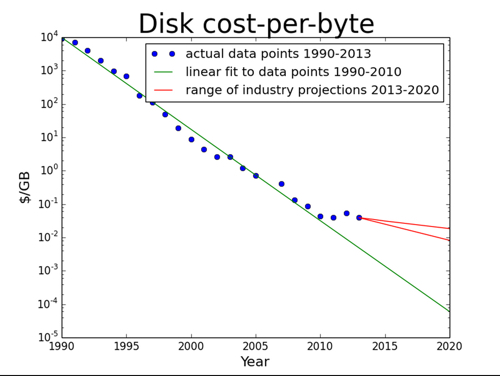
\includegraphics[width=0.75\textwidth]{img/kryder-slowdown}
\end{figure}

Een tweede kost waar er rekening mee moet worden gehouden zijn backups. Zoals vermeld in Hoofdstuk~\ref{sec:projections} zijn de databanken die gebruikt worden projecties van de afgebeelde events. Vermits deze een berekening zijn volstaat het om enkel van de events een backup te nemen, omdat de projecties opnieuw berekend kunnen worden\footnote{Er mag niet vergeten worden om een backup te nemen van data die niet in de databank wordt opgeslagen zoals afbeeldingen}.

\subsection{Developer kosten}
\label{subsec:developer-kosten}

Het is een andere manier van werken dus moeten de developers ook op de hoogte gebracht worden hoe ze met deze technologie moeten omgaan. Er zijn verschillende resources beschikbaar, waaronder https://eventsourcery.com. Zowel bij Skedify, als bij andere bedrijven wordt er gebruik gemaakt van OOP (Object oriented programming). EventSourcing gaat erg goed samen met functioneel programming omdat de huidige state een left fold is van vorige events.

\begin{equation}
\text{current state} = f(\text{events}, \text{action})
\end{equation}

Functioneel leren programmeren is dus een meerwaarde.

\subsection{Performance kosten}
\label{subsec:performance-kosten}

Telkens wanneer er een nieuwe command uitgevoerd wordt zoals vernoemd in Hoofdstuk~\ref{subsec:imperative-messages}, moeten alle events uit de EventStore overlopen worden om de huidige staat van het object op te bouwen. Dit wil zeggen dat bij elk nieuw event de applicatie trager zal worden. In kleine en middelmatige applicaties heeft dit geen gevolgen, naar grotere applicaties heeft dit grotere gevolgen. Hiervoor is een oplossing van snapshots. Een snapshot is de huidige state van een object na het overlopen van x aantal events. Deze kunnen in de EventStore opgeslagen worden, in een tabel naast de events zelf. Telkens wanneer de klasse beschrijving zou veranderen, moeten de snapshots opnieuw gegenereerd worden. Een tweede optie is om de current state ook op te slagen in memory, via deze weg moeten er geen events opnieuw afgespeeld worden om de huidige state van een object te kunnen bepalen omdat deze reeds beschikbaar is.